\section{Preprocessing Module}
Before starting writer recognition, a form needs to be analyzed to identify the handwritten area. For that purpose, we need to provide preliminary image pre-processing. The pre-processing algorithm includes mainly two steps:
\begin{enumerate}
  \item Handwritten Area Detection.
  \item Line Segmentation.
\end{enumerate}

\subsection{Handwritten Area Detection.}
The very first step of our algorithm to detect the writer of handwritten text is to detect and extract the handwritten area from the input image. It's noticed that all IAM database images have exactly three horizontal lines and The handwritten area is always contained between the second and the third lines. So when we talk about line detection, of course, we have to mention Hough Transform. 

Hough Transform is used widely to find imperfect instances of objects within a certain class of shapes by a voting procedure that is carried out in a parameter space of the required shape. By using Hough transform we were able to detect the three horizontal lines in IAM database forms and by ordering them by their \texttt{y} values in pixels, the two horizontal lines that contain the handwritten text can be easily detected as shown in Figure \ref{fig:preprocessing}. 

We used some heuristic values to be able to crop the handwritten area from the IAM database forms in case of Hough transform failure to detect the horizontal lines. we noticed that the lower line is always 2800 pixels down from the image top corner and the upper line is ranged from 550 to 700 pixels down from the upper corner. Finally, we cropped the image padding using 100 pixels from the left corner and 50 pixels from the right corner.

\begin{figure*}[h]
    \centering
    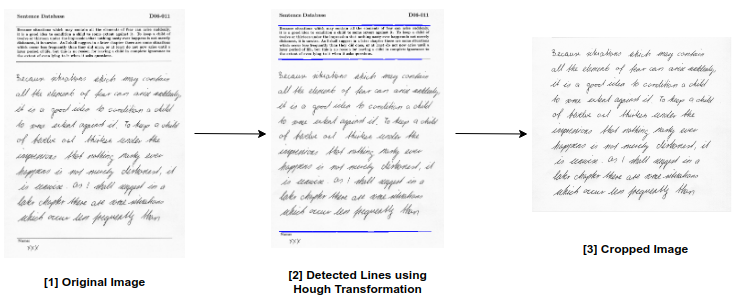
\includegraphics[width=\textwidth]{preprocessing}
    \captionof{figure}{Handwritten Area Detection}
    \label{fig:preprocessing}
\end{figure*}

\subsection{Line Segmentation.}
The second step in the preprocessing module is to segment the input form into a set of contours such that each contour represents one line of the handwritten text. This part depends mainly on morphological operations. It was divided into three main steps: 
\begin{enumerate}
  \item Image Dilation
  \item Image Opening.
  \item Find Contours.
\end{enumerate}

At first, we perform the morphological dilation operation using horizontal kernel on the cropped image from the previous part so that all words in the same line are merged in one single contour. 

We noticed that the dilated image has an overlapped lines merged as shown in Figure \ref{fig:segmentation}. So to solve this issue we performed the morphological opening operation using a vertical kernel so that we can remove all vertical lines from the image and separate the overlapped lines. 

Finally, we used  \texttt{openCV finCountours} function to extract the boundary boxes of the segmented lines and we add some margins above and down each line to compensate for the opening effect which may crop some pixels from the actual text line. 

\begin{figure*}[h]
    \centering
    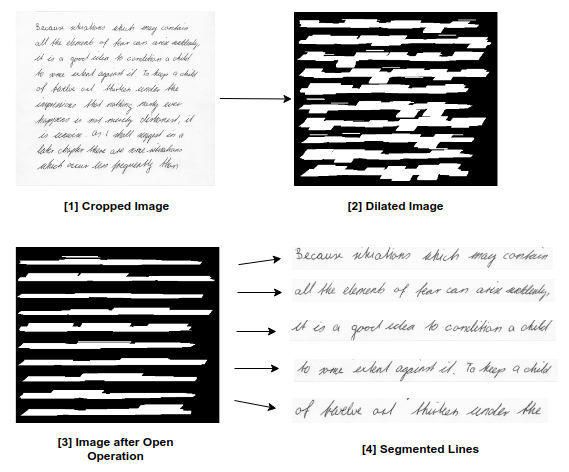
\includegraphics[width=\textwidth]{line-segmentation}
    \captionof{figure}{Line Segmentation}
    \label{fig:segmentation}
\end{figure*}